
\chapter{Preparation}
\section{The Mach-Zehnder Modulator}
\label{sec:MZM}
\begin{figure}[h]
  \centering
  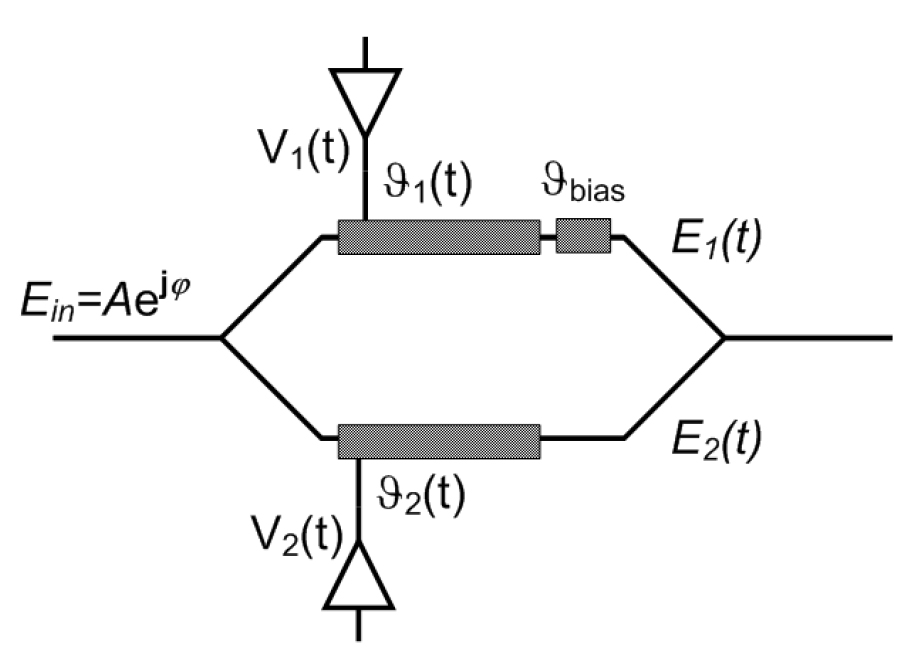
\includegraphics[width=.5\columnwidth]{Grafiken/Mach-Zehnder.jpg}

\caption{Setup of a Mach-Zehnder Modulator}
\label{fig:MZI}
\end{figure}
\begin{figure}[ht]
  \centering
  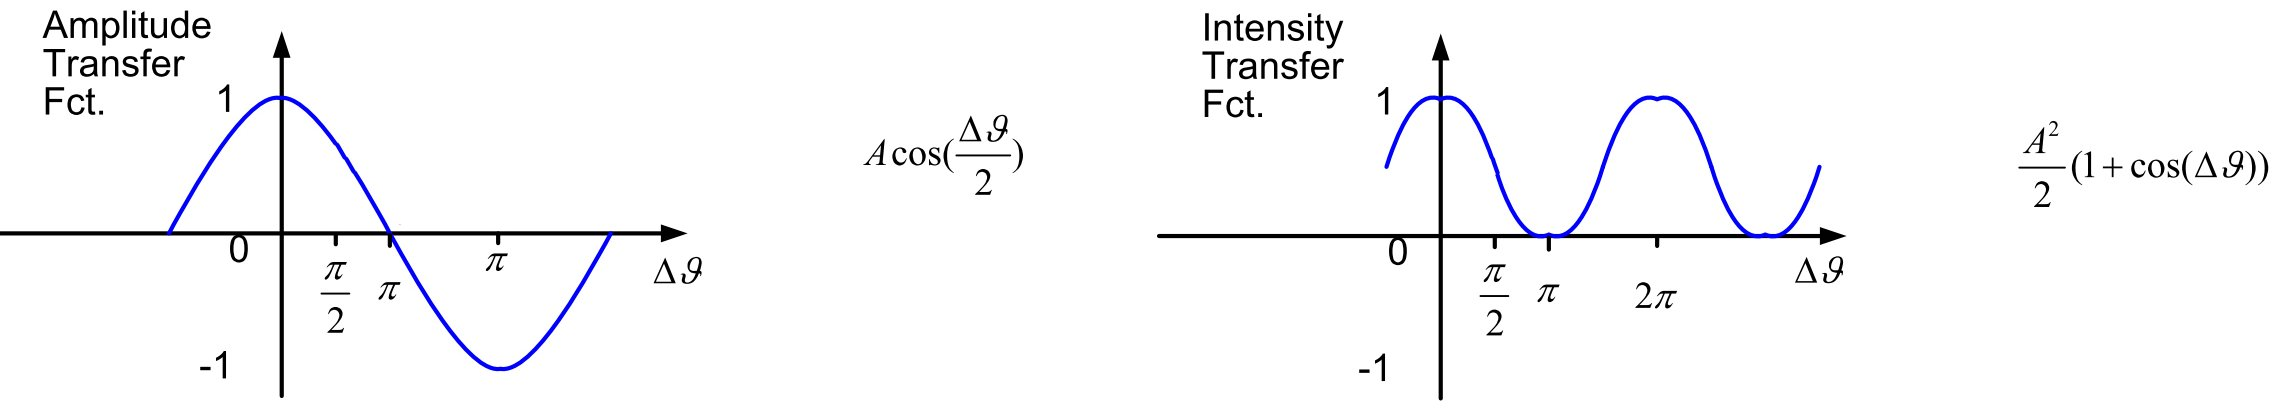
\includegraphics[width=\columnwidth]{Grafiken/Mach-Zender-Transfer1.jpg}

\caption{Amplitude tranfer function (left) and Intensity transfer function (right) of a Mach-Zehnder Modulator }
\label{fig:MZI_plot}
\end{figure}


In a Mach-Zehnder Modulator (MZM) the light is split up in two branches. In each branch there is a non-linear medium, through which the Phase of the Light can be shifted. At the end the Light is brought together, so that it is interfering. This setup is shown in Figure \ref{fig:MZI}. The Amplitude of the Field at the end of the Modulator can be expressed as:
\begin{equation}
 E_{\mathrm{out}}=\exp\left(j\frac{\vartheta_1+\vartheta_2}{2}+j\frac{\vartheta_{\mathrm{Bias}}}{2} \right)\cdot\cos\left(\frac{\vartheta_1-\vartheta_2}{2}+\frac{\vartheta_{\mathrm{Bias}}}{2}\right)\cdot E_{\mathrm{in}} .
\end{equation}
The phase shift of the Signal at the output of the modulator is described by the first term, the amplitude by the second term. For the phase Modulation $\vartheta_1 = \vartheta_2$ only the phase of the Signal is changed while the Amplitude stays constant. This operation mode is called "`push-push"' mode. For $\vartheta_1 = -\vartheta_2$ only the Amplitude of the Signal is modulated. This operation mode is called "`push-pull"' mode. \footnote[1]{Leuthold, J. : Optical Communication Systems. WS 2010/2011}



\section{Modulation Formats}
% \begin{figure}
%   \centering
% %   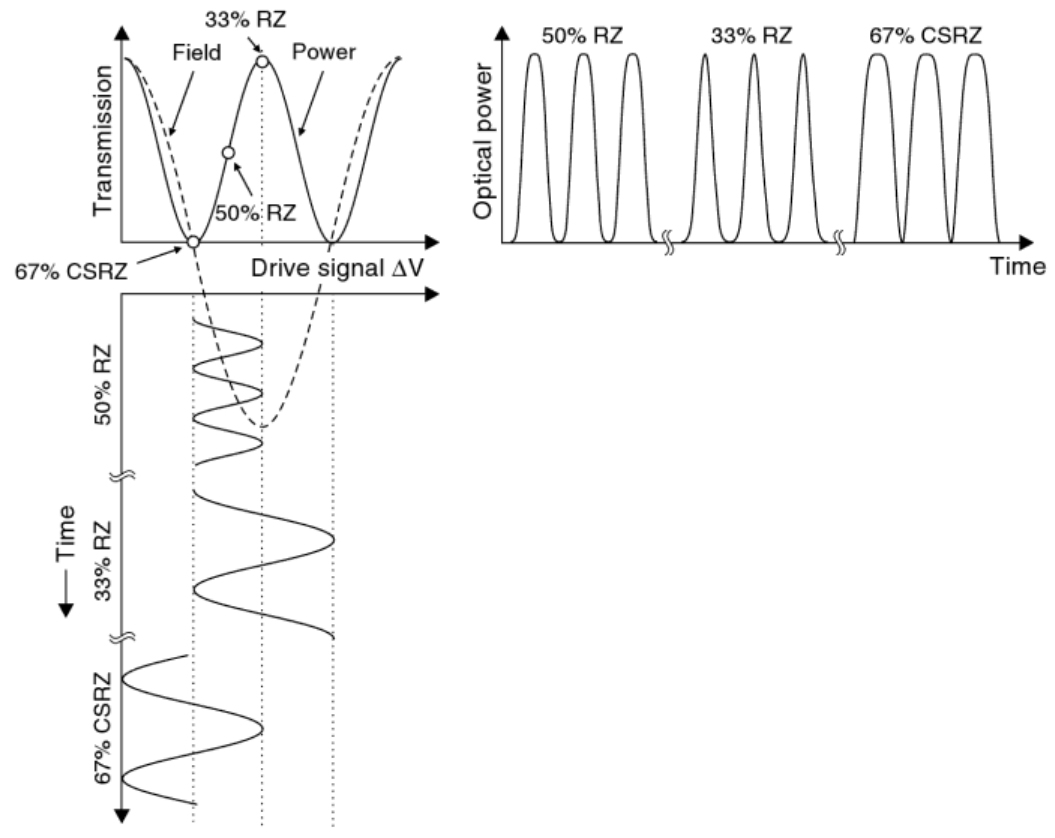
\includegraphics[width=.5\columnwidth]{Grafiken/RZ_OOK.jpg}
% % \caption{}
% % \label{fig:RZ_OOK}
% \end{figure}
% \begin{figure}
%   \centering
% %   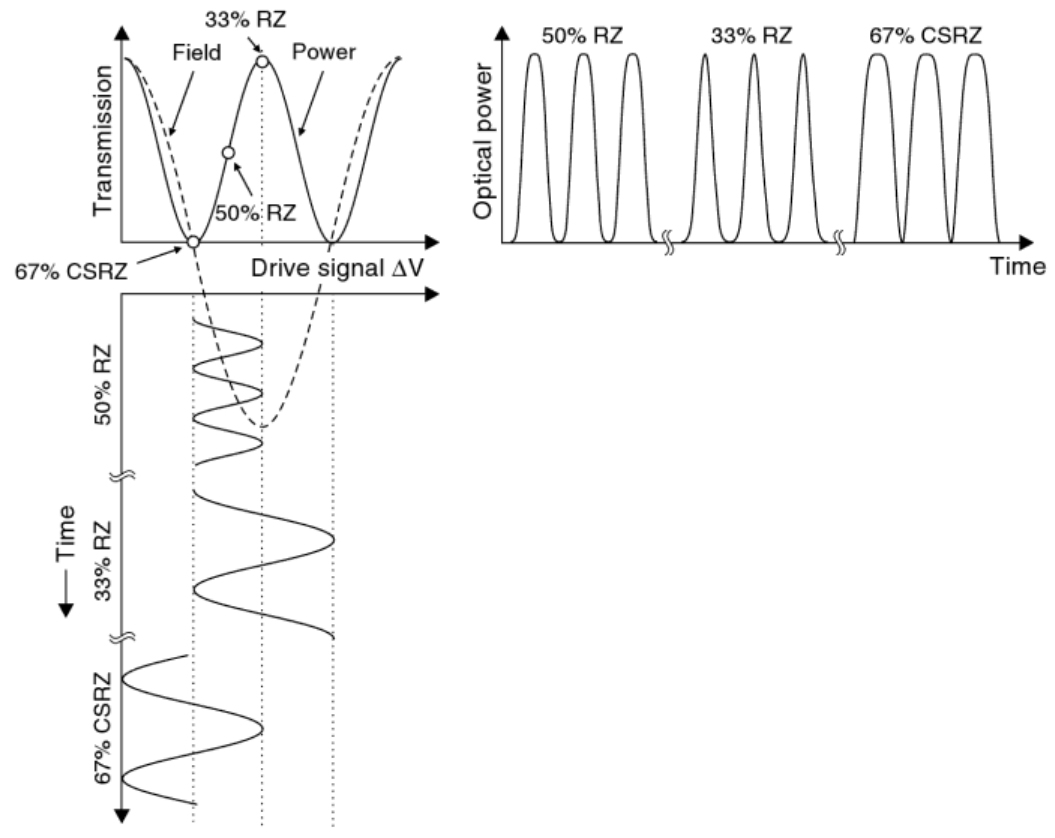
\includegraphics[width=.5\columnwidth]{Grafiken/RZ_OOK.jpg}
% % \caption{}
% % \label{fig:RZ_OOK}
% \end{figure}
% 



\subsection{Amplitude Shift Keying}
In Amplitude Shift Keying (AFK) information is transmitted by the amplitude of a signal. The level of the signal amplitude defines a binary value. In the case of "On/Off keying" (OOK) the binary symbol is "`0"' when there is no power transmitted. When there is power transmitted the symbol corresponds to a "`1"'. 
Figure \ref{fig:ask}a) shows such an ASK signal.\footnote[1]{Leuthold, J. : Optical Communication Systems. WS 2010/2011}

\begin{figure}
  \centering
  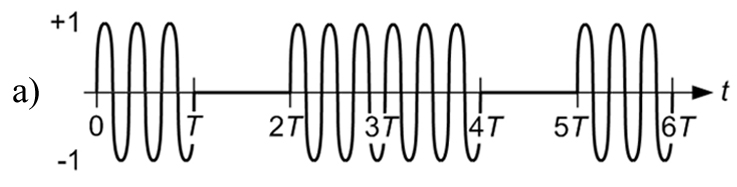
\includegraphics[width=.5\columnwidth]{Grafiken/OOK.jpg}
	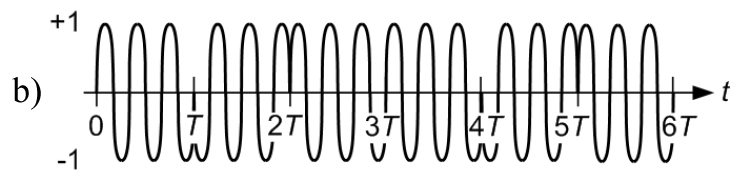
\includegraphics[width=.5\columnwidth]{Grafiken/PSK.jpg}%
\caption{\textbf{a)} Amplitude Shift Keying \textbf{b)} Phase Shift Keying}
\label{fig:ask}
\end{figure}

\subsection{Phase Shift Keying}
In Phase Shift Keying (PSK) information is transmitted by modulating the phase of a carrier wave. Because the amplitude and the freuency of a carrier wave is not changed, the intensity of the signal is constant and thus not influenced by non-linear effects. An example for a PSK modulated signal is shown in Figure \ref{fig:ask}b).\footnotemark[1]

\subsection{Quadrature Amplitude Modulation}
In Quadrature Amplitude Modulation (QAM) both the phase and the amplitude of a carrier wave is modulated. Thus it is possible to transmit multiple bits per symbol. The QAM signal is generated by summing multiple amplitude modulated signals that have a defined phase offset. For Multilevel modulation the number of symbols is usualy given (e.g. 16-QAM). In principle it is also possible to implement multiple Symbols with PSK and ASK, too. Note that there is no difference between QPSK and 4-QAM.\footnotemark[1]
\newpage
\section{Signal Generation}
\begin{figure}
  \centering
  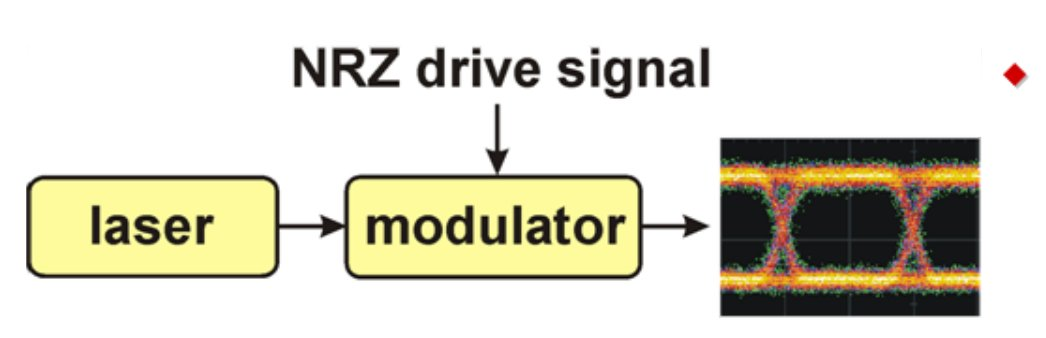
\includegraphics[width=.5\columnwidth]{Grafiken/Signal-generation.jpg}

\caption{Block diagram for the genaration of a OOK-/BPSK-Signal with a MZM }
\label{fig:signal}
\end{figure}

\subsection{Generation of a OOK-Signal}
A OOK-Signal for high-speed telecommunication systems is commonly created through external modulation of a MZM (cf. Figure \ref{fig:signal}). To do so the MZM is used in the push-pull operation mode. The switching voltage of the MZM varries between the zero transmission point and the amplitude maximum (cf. the handdrawn figure below). The resulting signal can be described as the superposition of the carrier wave and the modulating signal. \footnote[1]{Leuthold, J. : Optical Communication Systems. WS 2010/2011}
 %(cf. figure \ref{fig:signal_sup}).\footnotemark[1]
\subsection{Generation of a BPSK-Signal}
For the generation of a BPSK the same setup as for the OOK-Signal can be used. The MZM is also operated in the push-pull mode, but with twice the switching Voltage used for OOK modulation. This corresponds to the voltage between the minimum and the maximum of the transfer amplitude (cf. the handdrawn figure below).\footnotemark[1]
\newpage
\begin{figure}
  \centering
  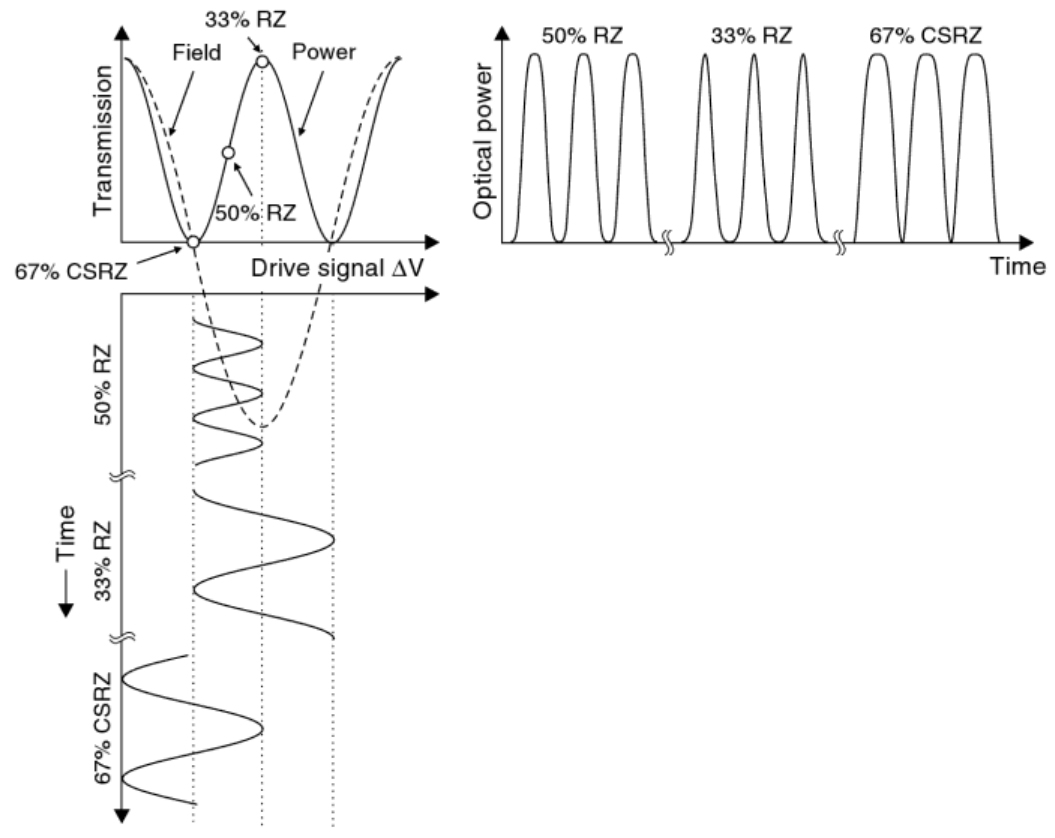
\includegraphics[width=.5\columnwidth]{Grafiken/RZ_OOK.jpg}
\caption{Different duty cycles for RZ signals}
\label{fig:RZ_OOK}
\end{figure}

\section{RZ Signal Generation}
\label{sec:RZ}
For the generation of a RZ signal, first a NRZ signal is created for example with one of the methods described above. Then another MZM is used to carve the signal into a RZ shape. It is possible to realize different pulse widths for the RZ signal. When the MZM is driven by a sine with the data rate between the minimum and the maximum of the transition the signal has a duty cycle of 50\%. When the MZM is driven by a sine with half the data rate between the minima of the transition the signal has a duty cycle of 33\%. When the MZM is driven by a sine with half the data rate between the maxima of the transition the signal has a duty cycle of 66\% (cf. figure \ref{fig:RZ_OOK}). Beside the lower pulse width and thus the lower power a 33\%-RZ signal has a larger spectral width than a 66\%-RZ signal. Furthermore the spectrum of a 66\%-RZ signal shows no peak at the carrier frequency and the spectral tones are at $\omega=\omega_0\pm2\pi\cdot R/2$.

This is a result of modulating the signal with $\omega_m=2\pi\cdot R/2$ in the push-pull mode. Because there is no additional unmodulated carrier added, the frequency $\omega_0$ is supressed in the spectrum. Through the modulation, neighboring bits have a phase difference of $\pi$. This means, that the "`1"' of a signal, are one half of the time positive, the other half of the time negative. This results in a zero mean signal. 
\comseb{bin nicht ganz zufrieden mit der formulierung}






\footnote[2]{Kaminow, I. P. ; Li, T. ; Willner, A. : Systems and Networks. Amsterdam :
Elsevier/Academic Press, 2008 (Optical Fiber Telecommunications V)}

